% mnras_template.tex 
%
% LaTeX template for creating an MNRAS paper
%
% v3.0 released 14 May 2015
% (version numbers match those of mnras.cls)
%
% Copyright (C) Royal Astronomical Society 2015
% Authors:
% Keith T. Smith (Royal Astronomical Society)

% Change log
%
% v3.0 May 2015
%    Renamed to match the new package name
%    Version number matches mnras.cls
%    A few minor tweaks to wording
% v1.0 September 2013
%    Beta testing only - never publicly released
%    First version: a simple (ish) template for creating an MNRAS paper

%%%%%%%%%%%%%%%%%%%%%%%%%%%%%%%%%%%%%%%%%%%%%%%%%%
% Basic setup. Most papers should leave these options alone.
\documentclass[fleqn,usenatbib]{mnras}

% MNRAS is set in Times font. If you don't have this installed (most LaTeX
% installations will be fine) or prefer the old Computer Modern fonts, comment
% out the following line
\usepackage{newtxtext,newtxmath}
% Depending on your LaTeX fonts installation, you might get better results with one of these:
%\usepackage{mathptmx}
%\usepackage{txfonts}

% Use vector fonts, so it zooms properly in on-screen viewing software
% Don't change these lines unless you know what you are doing
\usepackage[T1]{fontenc}
\usepackage{ae,aecompl}


%%%%% AUTHORS - PLACE YOUR OWN PACKAGES HERE %%%%%

% Only include extra packages if you really need them. Common packages are:
\usepackage{graphicx}	% Including figure files
\usepackage{amsmath}	% Advanced maths commands
\usepackage{amssymb}	% Extra maths symbols

%%%%%%%%%%%%%%%%%%%%%%%%%%%%%%%%%%%%%%%%%%%%%%%%%%

%%%%% AUTHORS - PLACE YOUR OWN COMMANDS HERE %%%%%

% Please keep new commands to a minimum, and use \newcommand not \def to avoid
% overwriting existing commands. Example:
%\newcommand{\pcm}{\,cm$^{-2}$}	% per cm-squared
\newcommand{\red}[1]{{\textcolor{red}{#1}}}
\newcommand{\green}[1]{{\textcolor{green}{#1}}}
\newcommand{\blue}[1]{{\textcolor{blue}{#1}}}

%%%%%%%%%%%%%%%%%%%%%%%%%%%%%%%%%%%%%%%%%%%%%%%%%%

%%%%%%%%%%%%%%%%%%% TITLE PAGE %%%%%%%%%%%%%%%%%%%

% Title of the paper, and the short title which is used in the headers.
% Keep the title short and informative.
\title[Decoupling the rotation of stars and gas - II]{Decoupling the rotation of stars and gas - II: black hole luminosity and the impact of feedback on large scale kinematics in IllustrisTNG}

% The list of authors, and the short list which is used in the headers.
% If you need two or more lines of authors, add an extra line using \newauthor
\author[C. Duckworth et al.]{Christopher Duckworth,$^{1,2}$\thanks{E-mail: cd201@st-andrews.ac.uk}
et al.
\\
% List of institutions
$^{1}$School of Physics and Astronomy, University of St Andrews, North Haugh, St Andrews, KY16 9SS, UK\\
$^{2}$Center for Computational Astrophysics, Flatiron Institute, 162 Fifth Avenue, New York, NY 10010, USA\\
}

% These dates will be filled out by the publisher
\date{Accepted XXX. Received YYY; in original form ZZZ}

% Enter the current year, for the copyright statements etc.
\pubyear{2019}

% Don't change these lines
\begin{document}
\label{firstpage}
\pagerange{\pageref{firstpage}--\pageref{lastpage}}
\maketitle

% Abstract of the paper
\begin{abstract}
We study the relationship between black hole (BH) feedback, BH luminosity and the large scale kinematics of stars and gas for galaxies in IllustrisTNG. We use a sample of galaxies with mock MaNGA observations at $z=0$ to identify kinematic misalignment, which we split on mass to separate the impact of `quasar' and `kinetic' feedback. 
Misaligned low mass galaxies (quasar feedback) typically have boosted BH luminosity, BH growth and have had more energy injected into the gas over the last 8 Gyr in comparison to aligned galaxies, which leads to outflows and gas loss.
Misaligned high mass galaxies (kinetic feedback) typically have similar BH luminosity over the last 8 Gyr with respect to aligned galaxies and show minimal gas loss. In particular, quenched galaxies shown no overall gas loss and have lower metallicity gas with respect to aligned galaxies, suggesting that the origin of misalignment is external.
We show that splitting on BH luminosity at $z=0$ produces statistically indistinct distributions of kinematic misalignment, indicative that despite a clear relationship between feedback and large scale kinematics, considering their correlation as an ensemble at a single time-step does not necessarily yield correlation.
\end{abstract}

% Select between one and six entries from the list of approved keywords.
% Don't make up new ones.
\begin{keywords}
galaxies: active -- galaxies: kinematics and dynamics -- galaxies: evolution
\end{keywords}

%%%%%%%%%%%%%%%%%%%%%%%%%%%%%%%%%%%%%%%%%%%%%%%%%%

%%%%%%%%%%%%%%%%% BODY OF PAPER %%%%%%%%%%%%%%%%%%

\section{Introduction}
Tidal torque theory \citep[][]{hoyle1951, peebles1969, Doroshkevich1970} dictates that the angular momentum content of collapsing baryons are inherited from the surrounding dark matter halo. In the framework of a $\Lambda$ cold dark matter Universe, galaxies form from the cooling and condensation of the initial gas cloud within dark matter haloes \citep{fall1980, mo1998}. As stars form from the rotating gas, 
% a natural expectation is that 
they inherit its dynamical characteristics leading to coherent rotation between dark matter, gas and stars in both magnitude and direction. However, after turnaround there is good reason to believe that the rotation of dark matter, gas and stars may decouple from each other as galaxies evolve up-to $z=0$. 

Recent cosmological scale hydro-dynamical simulations have provided a clear insight into the nature of the relationship between the angular momentum of baryons and dark matter through cosmic time. A necessary component of realistic simulations is efficient feedback from both black holes (BH) and stars, required to, amongst other things, reproduce late type disks and solve the problem of catastrophic angular momentum loss \citep[e.g.][]{zavala2008, scannapieco2009}. Active galactic nuclei (AGN) and supernova explosions can also lead to dramatic redistribution of gas which regulate the angular momentum content of galaxies \citep[e.g.][]{genel2015, DeFelippis2017}. 
% Galactic winds carry both mass and angular momentum leading to potential boosts in angular momentum \citep[e.g.][]{genel2015, DeFelippis2017}. 

The exact impact of black holes on angular momentum is dependent on the mode of feedback. `Quasar' (radiative) mode feedback releases huge amounts of energy through radiation from the accretion disk leading to high luminosity AGN and dramatic gas outflows \citep[e.g.][]{cattaneo2009, rubin2014, cheung2016}. Alternatively `radio' (kinetic) mode is termed for lower luminosity AGN that host lower black hole accretion rates. In this instance energy is deposited into the surrounding gas via jets and winds which heat the gas and suppress star formation \citep[][]{binney1995, ciotti2001, heckman2014}.

The relationship between AGN and kinematics has been the focus of several recent studies using Integral Field Spectroscopy (IFS) data. In particular, a new class of galaxy termed `red geyser' has been identified which host AGN and exhibits high velocity outflows in the spatial distribution of ionized gas \citep[][]{cheung2016, roy2018}. These outflows are often linked to a distinctive offset in rotation direction between the stars and gas. However detection of ongoing outflows is rare ($\sim5-10$\% of the quiescent population). \citet{penny2018} demonstrate the importance of AGN feedback in low mass quiescent galaxies. While the majority demonstrate no ionized gas present, quiescent galaxies with an active AGN that is actively suppressing star formation show a clear decoupling in the rotation of stars and gas. However, the relationship of large scale gas kinematics to BH feedback is not clear for all galaxies. \citet{ilha2019} find that typical rotation offsets between stars and gas for AGN defined galaxies are consistent with inactive controls. Termed kinematic misalignment, the decoupled rotation of stars and gas can also be a natural result of external processes \cite[e.g.][]{davis2011, barrera2015, vdvoort2015, jin2016}. Regardless of internal or external origin, kinematic misalignment is linked with both typical lower gas mass fractions and angular momentum \citep[e.g. Duckworth et al.,][]{starkenburg+19}. 

% Recent studies have shown a strong relationship between visual morphology and the likelihood of misalignment \citep[e.g. Duckworth et al. submitted,][]{chen2016, bryant2019}. Properties such as stellar mass are different when comparing aligned and misaligned galaxies of the same morphology and the difference (whether positive or negative) is morphologically dependent. Misaligned early-type galaxies are more massive, whereas misaligned late-types are less massive when compared to their aligned controls. This could be an indication that whether the misalignment is internally or externally driven is also morphologically dependent. \red{not relevant}

Misalignment appears to be ubiquitous in galaxies with ongoing feedback and outflows (that still have gas), however, the timescales of luminous AGN are typically much shorter than kinematic misalignment, making correlation at $z=0$ alone difficult. In this letter, we study the time evolution relationship between black hole feedback, black hole luminosity and kinematic misalignment in the cosmological scale hydrodynamical simulation of IllustrisTNG100 (hereafter referred to as TNG100). We use a sample of galaxies with mock MaNGA \citep[Mapping Galaxies at Apache Point;][]{bundy2015, blanton2017} observations at $z=0$ to emulate what we may expect to see in IFS observations. In Section \ref{sec:methods} we briefly describe the simulation and how we construct our sample. In Section \ref{sec:results} we present our results before concluding in Section \ref{sec:conclusion}.

\section{Methods} \label{sec:methods}
For this work, we use the fiducial run of TNG100 which follows the evolution of 2 x 1820$^3$ resolution elements within a periodic cube with box lengths of 110.7 Mpc (75 h$^{-1}$ Mpc). This corresponds to an average mass resolution of baryonic (dark matter) elements of 1.4 x 10$^6 M_{\odot}$ (7.5 x 10$^6 M_{\odot}$). The IllustrisTNG project \citep{marinacci18,naiman18,nelson18,pillepich18b,springel18} is a suite of magneto-hydrodynamic cosmological scale simulations incorporating an updated comprehensive model for galaxy formation physics \citep[][]{weinberger17,pillepich18a} and making use of the moving-mesh code \texttt{AREPO} \citep{springel10,pakmor11,pakmor13}. We make use of public data \citep[as described in][]{nelson2019}. Of particular relevance is the prescription of \citet{weinberger17} for BH feedback. As in other simulations \citep[e.g.][]{dubois2016}, AGN feedback is modelled by two modes (quasar mode: high accretion, kinetic mode: low accretion). The transition between modes is dictated by both the BH mass and accretion rate onto the BH, so that as BHs grow over time the kinetic mode is likely to become more dominant. 
% We note that in the kinetic model, the direction of injected momentum is random. 

To emulate what we may expect to see in IFS observations we construct a sample of TNG100 galaxies with mock MaNGA observations. 
% Set to complete in 2020, the MaNGA survey is designed to investigate the internal structure of $\sim$10000 galaxies in the nearby Universe. By design, the complete sample is unbiased towards morphology, inclination and colour and provides a near flat distribution in stellar mass. 
For each MaNGA galaxy, we find an object in TNG100 with the closest match in stellar mass, $g-r$ colour and size. We define the degree of misalignment between the rotation of stars and gas by fitting a position angle (PA) to the mock MaNGA velocity fields using the \texttt{fit\_kinematic\_pa} routine \citep[see Appendix C of][]{krajnovic2006} so that $\Delta PA = |PA_{stellar} - PA_{H\alpha}|$. We take objects with $\Delta$PA < 30$^{\circ}$ to be aligned, $\Delta$PA > 30$^{\circ}$ to be misaligned and $\Delta$PA > 150$^{\circ}$ to be counter-rotating. For a complete description of the construction of this sample, mock observations and PA fitting we direct the reader to Duckworth et al. We use $\sim$3600 galaxies with defined $\Delta$PAs in this work. 

\section{Results} \label{sec:results}
\begin{figure*}
	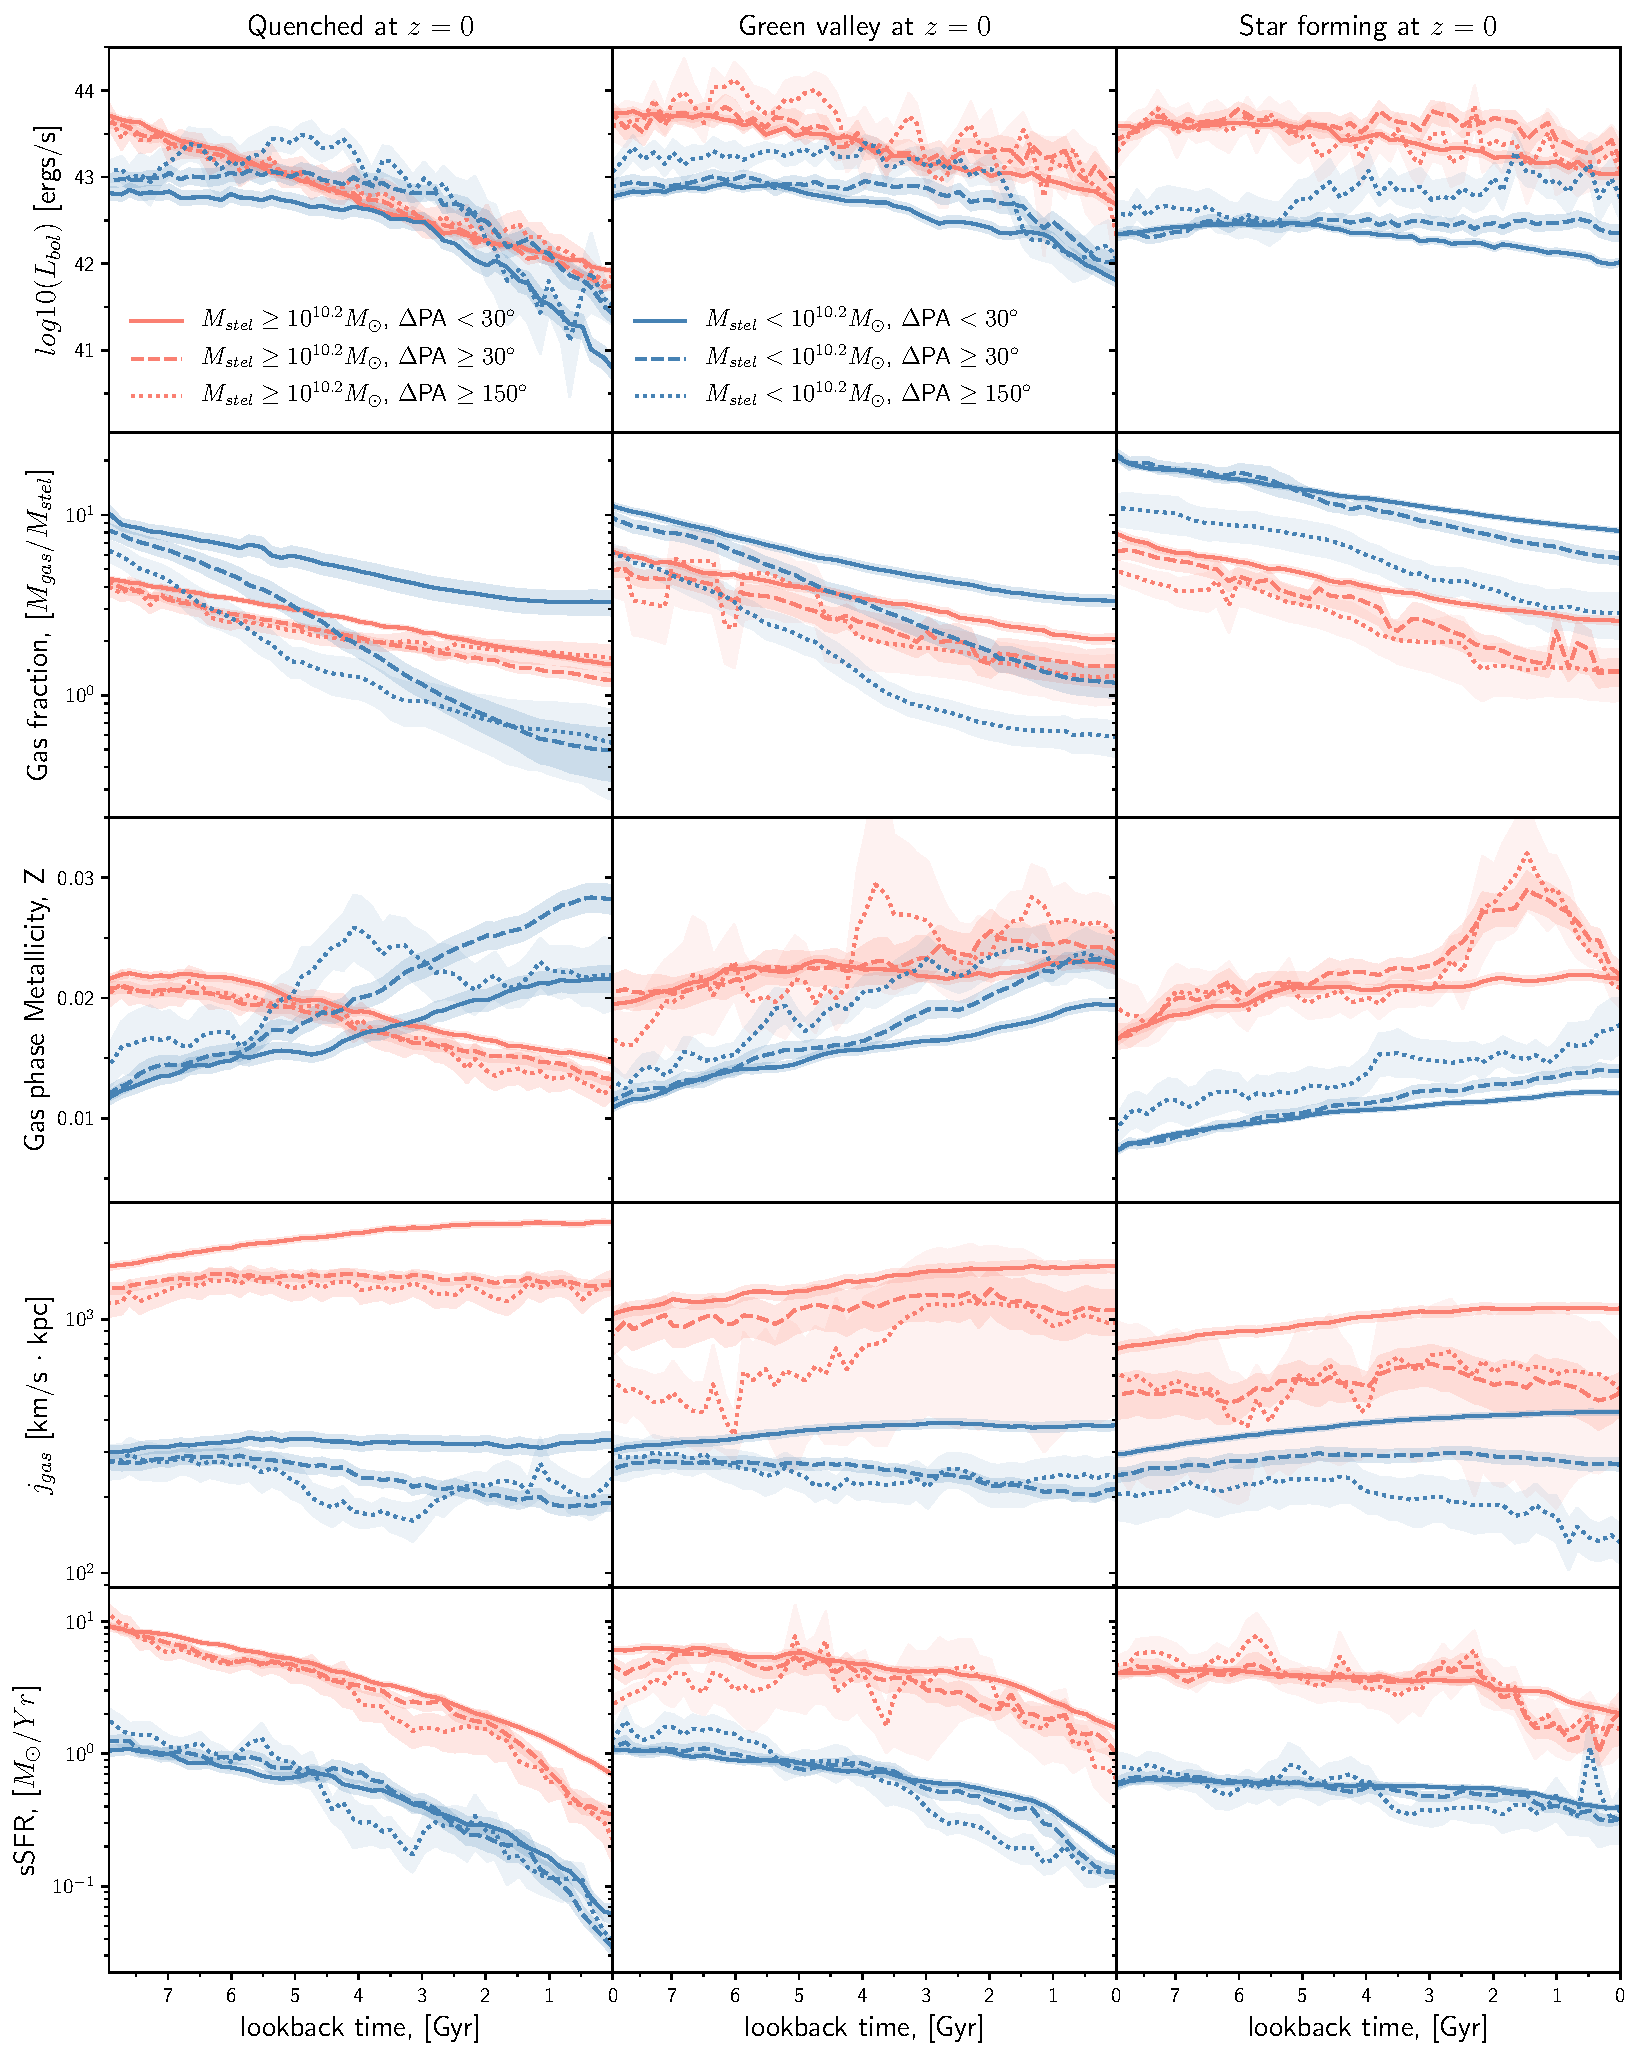
\includegraphics[width=0.65\linewidth]{overall_population/overall_pop_evolution_Mstel10_2.pdf}
    \caption{Time evolution of (rows top to bottom) black hole luminosity ($log_{10}(L_{bol})$), gas fraction ($M_{gas}$/$M_{stel}$), gas angular momentum ($j_{gas}$), gas phase metallicity and specific star formation rate for (columnns left to right) quenched, green valley and star forming galaxies identified at $z=0$. In each panel, the time evolution is split at $M_{stel} = 10^{10.2}M_{\odot}$ (corresponding to the transition from quasar to kinetic feedback) and also $\Delta$PA $< 30^{\circ}$ (solid) and $> 30^{\circ}$ (dashed) and  $> 30^{\circ}$ (dotted). Each line shows the mean for the population with the shaded region corresponding to the standard error.}
    \label{fig:overall_pop}
\end{figure*}

Each panel of Figure \ref{fig:overall_pop} shows the time evolution average of a property for all galaxies split by stellar mass at $M_{stel} = 10^{10.2}M_{\odot}$. This corresponds to the typical transition from quasar to kinetic feedback \citep[i.e. $M_{BH} \approx 10^{8}M_{\odot}$, see Fig 1 in][]{li2019}. We note that splitting on BH mass or enforcing stricter stellar mass cuts does not change any of our findings. We also divide our sample by $\Delta$PA (< 30$^{\circ}$ - solid, > 30$^{\circ}$ - dashed, > 150$^{\circ}$ - dotted) at $z=0$. Columns (left to right) show the evolutions of quenched, green valley and star forming galaxies individually \cite[defined by deviation from the star forming main-sequence in][]{pillepich2019}. 

In the top row we see distinct correlations between $\Delta$PA at $z=0$ and BH luminosity ($log_{10}(L_{bol})$) in the last 8 Gyr for low mass galaxies. This is most apparent for those that are counter-rotating at $z=0$, however a boost can be seen for all misaligned galaxies. In contrast, we note that the correlation between misalignment and AGN luminosity for the high mass bin is unclear. Since low (high) mass galaxies in TNG100 exhibit `quasar' (`kinetic') mode feedback, a possible interpretation is that quasar mode feedback is more likely to lead to misaligned gas rotation. For low mass galaxies, gas loss is a key feature (second row - defined for all gas associated with the galaxy), potentially indicative of gas outflows from the feedback which also lower the angular momentum content of the gas (fourth row - defined for gas within a 3D radius of the IFS observational footprint). This is also matched by a boost in gas phase metallicity (third row - all gas).

In contrast, for the high mass quenched galaxies we find that the gas fraction for the misaligned remains constant with respect to those aligned and the gas phase metallicity is typically lower. This is indicative that accretion (of pristine gas) and gas rich minor mergers is potentially more important for decoupling their rotation. This could be a natural result of quenched galaxies hosting smaller gas reservoirs, meaning that only a small amount of accretion (relatively to late-types) leads to misalignment. Interestingly, the angular momentum content of the gas is disrupted to a similar degree as for quasar feedback. 

In the bottom row, we see that the specific star formation rate (sSFR - all gas) typically decreases for misaligned galaxies in the last few Gyrs (before $z=0$) in comparison with the aligned. Regardless of the mechanism leading to misalignment, a slight suppression of sSFR is a common theme.

\begin{figure*}
	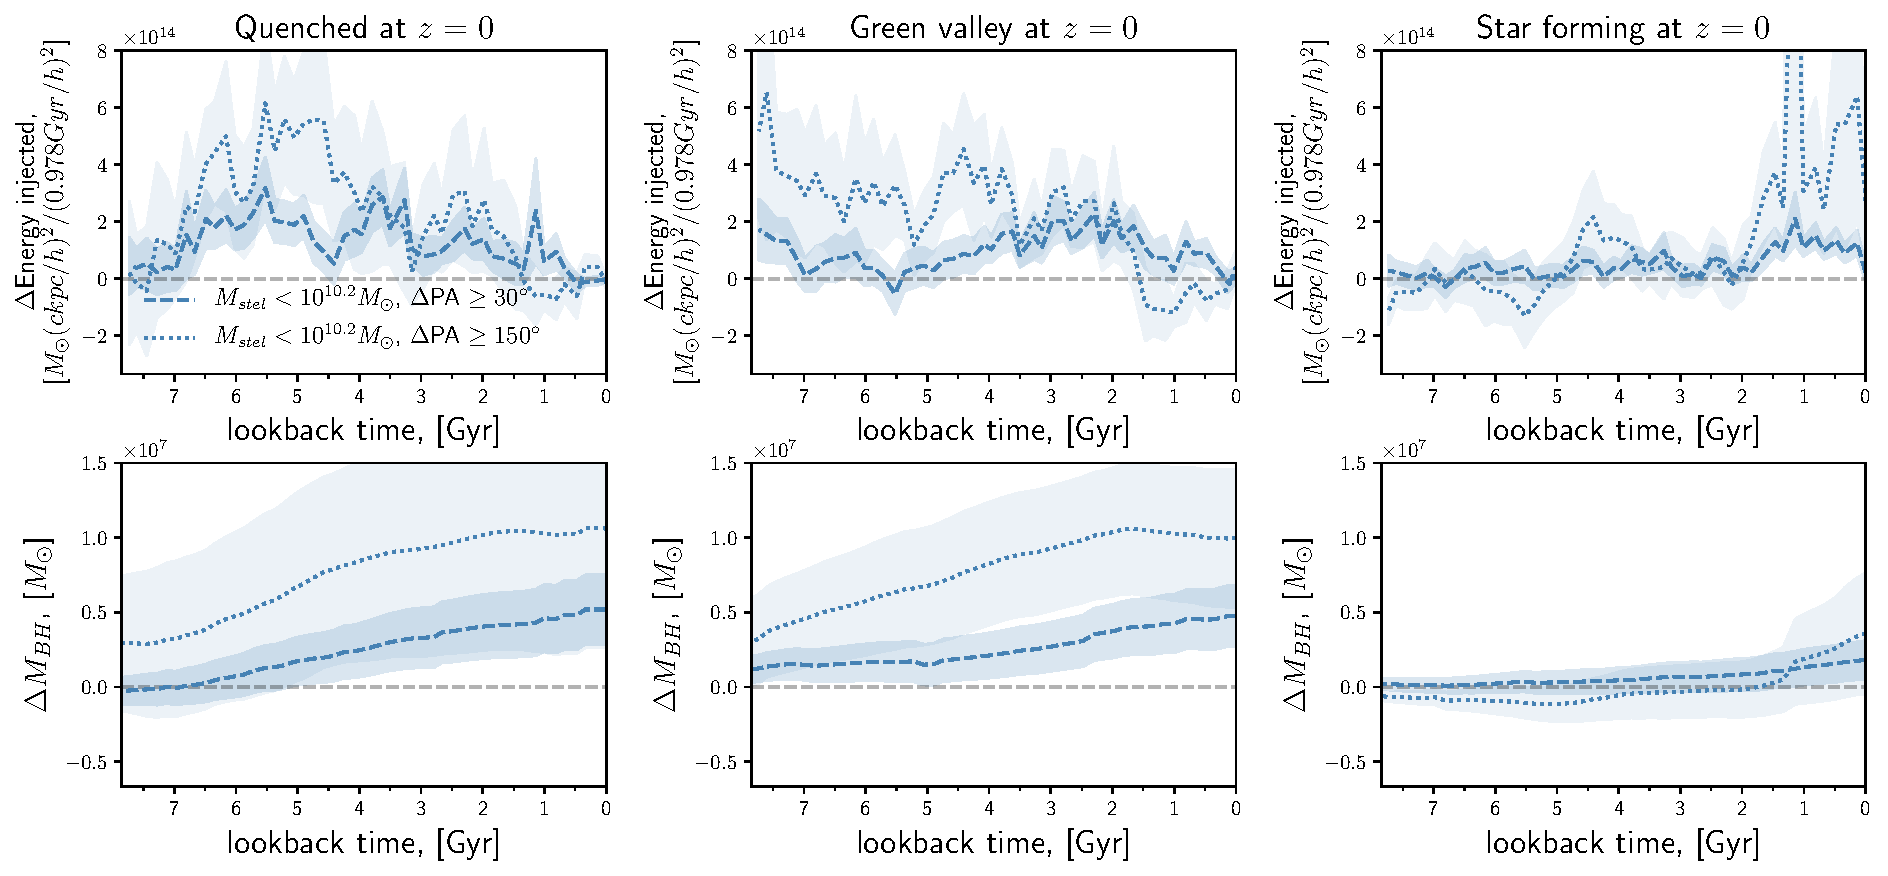
\includegraphics[width=0.9\linewidth]{overall_population/LM_BH_residual_evo_Mstel10_2.pdf}
    \caption{Time evolution of black hole energy injection (top; see main text for more detail) and black hole mass (bottom) for (columnns left to right) quenched, green valley and star forming galaxies identified at $z=0$. Shown are residuals for the bottom 33\% in stellar mass for $\Delta$PA$ > 30^{\circ}$ (dashed) and $\Delta$PA$ > 150^{\circ}$ (dotted) defined relative to $\Delta$PA$ < 30^{\circ}$. Each line shows the mean for the population with the shaded region corresponding to the standard error.}
    \label{fig:LM_BH}
\end{figure*}

To better understand the relationship between misalignment and BH feedback in low mass galaxies, in Figure \ref{fig:LM_BH} we show the time evolution of energy injection into the surrounding gas cells and black hole mass (see supplementary material for high mass equivalent of this plot). For these properties we plot the average residual difference of misaligned (dashed) and counter-rotating (dotted) galaxies with respect to the aligned galaxies (grey dashed line at the origin). We find that the rate of energy injection is richer for low mass counter-rotating galaxies, however a boost can be seen for all those that are misaligned. Interestingly the lookback time at which feedback energy injection peaks appears to be different as a function of morphology. Star forming galaxies show far more recent feedback and BH luminosity, indicative that while the gas is in the process of being decoupled and blown out, it hasn't acted to fully quench the galaxy yet. Conversely, looking at green valley and quenched galaxies we can see that the feedback starts earlier allowing for the drop in SFR we see today. This can also be seen, to a lesser degree, for the BH luminosity evolution. 

We also show the residual time evolution of black hole mass with respect to the aligned galaxies. For all low mass galaxies, we see a steady divergence of misaligned galaxies from the aligned control as black hole mass difference increases over time. As we see that angular momentum is disrupted in misaligned galaxies, it may be natural to think that this leads to an increased inflow of gas into the galaxy centre and hence black hole.

\begin{figure}
	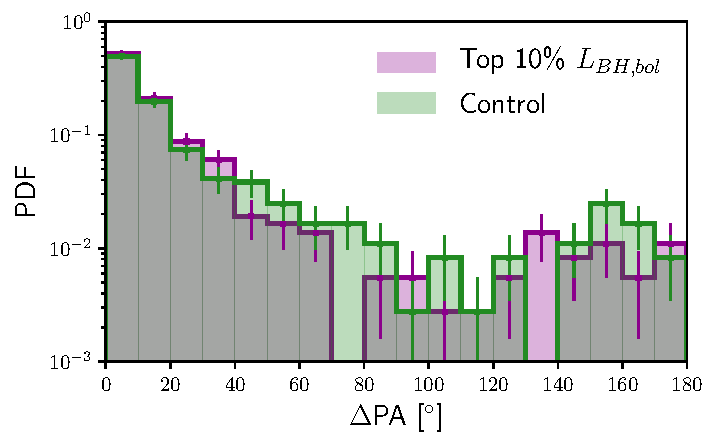
\includegraphics[width=0.9\linewidth]{overall_population/PA_distribution_BHlum_split.pdf}
    \caption{Probability density distributions of kinematic misalignment as defined by $\Delta$PA at $z=0$. Shown are the brightest 10\% AGN in our sample (also defined at $z=0$, purple) compared with a mass matched control sample (green). Despite the relationship between BH luminosity and kinematic misalignment, this demonstrates that considering the distributions at a single time-step does not necessarily yield correlation. This holds true if these distributions are made and compared for star-forming, green-valley and quenched galaxies only.}
    \label{fig:PAdist}
\end{figure}

In Figure \ref{fig:PAdist}, we show the distribution of $\Delta$PA for the top 10\% BH luminosity in our sample in comparison with a control (all defined at $z=0$). The control is made by taking the closest unique match in stellar mass for each high BH luminosity galaxy from the remainder of our sample. We find the two distributions are statistically indistinct (Kolmogorov--Smirnov test; 0.06 with a p-value of 0.38). This demonstrates, despite the inherent relationship between BH luminosity, feedback and gas kinematics, considering the overall distribution of $\Delta$PA split on luminosity at a single time-step does not necessitate that correlation is found. Feedback is a clear mechanism for driving misalignment, however the decoupled rotation of gas can remain for several Gyr after initially becoming misaligned, meaning that a single time-step is unlikely to characterise the relationship for an ensemble of galaxies. 

We note that IllustrisTNG typically under-produces bright AGN ($L_{BH} > 10^{44}$ergs$^{-1}$) for $z \leq 1$ in contrast with observational constraints \citep[see][]{habouzit2019}. Given this and the uncertainty in estimating BH luminosity, we chose to select by percentile rather than cutting on absolute luminosity. Regardless, selecting only bright AGN in this way does not change our findings.

\section{Summary} \label{sec:conclusion}
In this paper, we study the relationship between BH luminosity, BH feedback and kinematic misalignment between stars and gas for galaxies in IllustrisTNG. We use mock observations of an IFS survey (MaNGA like) built from galaxies in TNG100, to identify kinematic misalignment ($\Delta$PA; difference in PAs of stars and gas) at $z=0$. We split our mock IFS sample on morphology and mass ($M_{stel} = 10^{10.2}M_{\odot}$) to separate the impact of `quasar' and `kinetic' feedback modes. We follow the time evolution of BH luminosity and energy injection from BH feedback in leading up to misalignment (or counter-rotation) between the star and gas kinematics at $z=0$. We compare the $z=0$ distributions of $\Delta$PA of the most luminous BHs in our sample against a control. Our conclusions are as follows.
\begin{enumerate}
    \item Low mass galaxies (quasar mode feedback) with misalignment (and counter-rotation) at $z=0$ typically have boosted BH luminosity, BH growth and have had significantly more energy injected into the gas over the last 8 Gyr in comparison to aligned galaxies. Gas (all phases) outflows due to the feedback, losing angular momentum increasing metallicity towards $z=0$. This is seen for all populations split on $z=0$ sSFR.
    \item The epoch of peak energy injection from the quasar mode feedback is different as a function $z=0$ sSFR for misaligned galaxies. This epoch is earlier for lower $z=0$ sSFRs and later for higher $z=0$ sSFRs. This is a natural consequence of lower sSFR galaxies being exposed to more violent feedback on longer timescales and hence having a smaller amount of star forming gas at $z=0$. 
    \item High mass galaxies (kinetic mode feedback) with misalignment (and counter-rotation) at $z=0$ typically have similar BH luminosity over the last 8 Gyr with respect to aligned galaxies and gas loss, if any, is less dramatic. In particular, we note that misaligned quenched galaxies show no gas loss in the last 8 Gyr and typically have lower gas phase metallicity (with respect to aligned galaxies). This suggests that the origin of misalignment in massive ETGs is more likely due to accretion of pristine gas.
    \item We find that the distributions of kinematic misalignment are statistically indistinct between the top 10\% in BH luminosity of galaxies in our sample and a mass matched control at $z=0$. This matches observations \citep[see Figure 6 in][]{ilha2019} and demonstrates that despite a clear relationship between feedback and large scale kinematics, considering their correlation as an ensemble at a single time-step does not necessarily yield correlation.
\end{enumerate}
The timescales of star-gas misalignment are of the order Gyrs and are dependent on the strength of the stellar torque in the galaxy. In addition, counter-rotation is a stable state and hence stars and gas can continue to remain decoupled. Further study is required to determine the exact origin of decoupled rotation in observations as a function of morphology. Regardless, this work demonstrates the importance of feedback for low mass galaxies on large scale kinematics and points to an external origin of misalignment for massive ETGs.

\section*{Acknowledgements}
CD acknowledges support from the Science and Technology Funding Council (STFC) via an PhD studentship (grant number ST/N504427/1) and from the Simons Foundation through its support of the Flatiron Institute. We thank the IllustrisTNG team; while this work was conducted using the public data release, it would have not been possible without use of the private data for the purposes of other research works. 

%%%%%%%%%%%%%%%%%%%%%%%%%%%%%%%%%%%%%%%%%%%%%%%%%%

%%%%%%%%%%%%%%%%%%%% REFERENCES %%%%%%%%%%%%%%%%%%

% The best way to enter references is to use BibTeX:

\bibliographystyle{mnras}
\bibliography{biblio} 

%%%%%%%%%%%%%%%%%%%%%%%%%%%%%%%%%%%%%%%%%%%%%%%%%%


% Don't change these lines
\bsp	% typesetting comment
\label{lastpage}
\end{document}

% End of mnras_template.tex